\documentclass[a4paper,11pt]{article}
% Various packages
\usepackage{siunitx}
\usepackage[utf8]{inputenc} % æøå
\usepackage[T1]{fontenc} % mere æøå
\usepackage[danish]{babel} % orddeling
\usepackage{verbatim} % så man kan skrive ren tekst
\usepackage{graphicx}
\graphicspath{{assets/}}
\usepackage{a4wide}
\usepackage{url}
\usepackage[left=2cm,top=2cm,bottom=1.5cm,right=2cm]{geometry}
\usepackage{amsmath}
\usepackage{amssymb}
\usepackage{amsthm}
\usepackage{wrapfig}
\usepackage{fixme}
\usepackage{color}
\usepackage[makeroom]{cancel}
\usepackage{pstricks}
\usepackage{pdfpages} % include pdf
\usepackage{forest}
\usepackage{float} % Use [H] in figures
\usepackage{subcaption} % For subfigures
\usepackage{color} % May be necessary if you want to color links
%\usepackage{xcolor} \pagecolor[rgb]{0,0,0} \color[rgb]{1,1,1}
\usepackage{nameref}
\usepackage{hyperref} % Make references clickable
\usepackage[nameinlink,capitalize]{cleveref} % Make eq:refs be in style (1)
\usepackage[linesnumbered, commentsnumbered, lined, ruled, vlined,
%noend  % Have no ⌊-like symbol to indicate end of scope in pseudocode
]{algorithm2e} % Doc: https://goo.gl/6bC1qZ

\crefname{equation}{}{Equations}

% Ændr på navnene der vises når man bruger \autoref{label}
\def\sectionautorefname{Sektion}
\renewcommand{\equationautorefname}{Ligning}
\def\figureautorefname{Figur}
\AtBeginDocument{\renewcommand{\ref}[1]{\autoref{#1}}}

% Sæt \ref{} til at kalde \autoref{}
\AtBeginDocument{\renewcommand{\ref}[1]{\autoref{#1}}}

% Ændr ''*'' i math-felter til \cdot
\DeclareMathSymbol{*}{\mathbin}{symbols}{"01}

% Sæt farver for interne referencer og links
\definecolor{darkblue}{RGB}{25,25,112}
\hypersetup{
	colorlinks=true,    %set true if you want colored links
	linktoc=all,        %set to all if you want both sections and subsections linked
	linkcolor=darkblue, %choose some color if you want links to stand out
	filecolor=blue,     %
	citecolor=black,    %
	urlcolor=cyan,      %
}

% Set indentation to 0:
\setlength\parindent{0pt}

% Keywords relateret til algorithm2e pakken
\newcommand{\True}{\textbf{true}}\newcommand{\False}{\textbf{false}}
\SetStartEndCondition{ }{}{}%
\SetKwProg{Fn}{def}{\string:}{}
\SetKw{KwTo}{to}
\SetKwFor{For}{for}{}{}%
\SetKwFor{ForEach}{foreach}{}{}%
\SetKwIF{If}{ElseIf}{Else}{if}{}{elif}{else}{end}%
\SetKwFor{While}{while}{}{end}\SetKwProg{Fn}{}{}{}
\SetKwInOut{Input}{input}\SetKwInOut{Output}{output}
\setlength{\algomargin}{3em}\DontPrintSemicolon

\newcommand{\longspace}{{\ \ \ \ \ \ \ \ \ \ \ \ \ \ }}
% \renewcommand{\P}{{\mathbb P}}
\newcommand{\R}{{\mathbb R}}
\newcommand{\E}{{\mathbb E}}
\newcommand{\event}{{\mathcal{E}}}
\newcommand{\parfrac}[1]{\frac{\partial}{\partial #1}}
\renewcommand{\num}{{\textrm{num} }}
\newcommand{\size}{{\textrm{size} }}
\newcommand{\ift}{{\textrm{if } }}

\newcommand{\pfrac}[2]{\left( \frac{#1}{#2} \right)}

% Dynamiske (), <>, ceil, floor
\newcommand{\p}[1]{\left( #1 \right)}
\newcommand{\pbig}[1]{\big( #1 \big)}
\newcommand{\pBig}[1]{\Big( #1 \Big)}
\newcommand{\pbigg}[1]{\bigg( #1 \bigg)}
\newcommand{\curly}[1]{\left\{ #1 \right\}}
\renewcommand{\square}[1]{\left[ #1 \right]}
\newcommand{\larr}[1]{\left< #1 \right>}
\newcommand{\ceil}[1]{\left\lceil #1 \right\rceil}
\newcommand{\floor}[1]{\left\lfloor #1 \right\rfloor}

\renewcommand{\P}[1]{\mathbb{P} \square{ #1 } }

\author{Søren Mulvad, rbn601}

\title{Eksamensdisposition - Algebraiske Teknikker}

\begin{document}
\maketitle

\begin{itemize}
  \item \textbf{Freivalds teknik: Matrixprodukt verificering}
  \item \textbf{Freivalds teknik: Polynomial identitet}
  \item \textbf{Schwartz-Zippel Theorem: Multivariabel polynomial identitet}
  \item \textbf{Streng-lighed 1: (mod p) fingerprint}
  \item \textbf{Streng-lighed 2: Freivald (Polynomier)}
  \item \textbf{Pattern Matching: Efficient Fingerprints}
\end{itemize}


%%%%%%%%%%%%%%%%%%%%%%%%%%%%%%%%%%%%%%%%%%%%%%%%%%%%%%%%%%%
%%%%%%%%%%%%%%%%%%%%%%%%%%%%%%%%%%%%%%%%%%%%%%%%%%%%%%%%%%%
%%%%%%%%%%%%%%%%%%%%%%%%%%%%%%%%%%%%%%%%%%%%%%%%%%%%%%%%%%%
\newpage
%%%%%%%%%%%%%%%%%%%%%%%%%%%%%%%%%%%%%%%%%%%%%%%%%%%%%%%%%%%
%%%%%%%%%%%%%%%%%%%%%%%%%%%%%%%%%%%%%%%%%%%%%%%%%%%%%%%%%%%
%%%%%%%%%%%%%%%%%%%%%%%%%%%%%%%%%%%%%%%%%%%%%%%%%%%%%%%%%%%
\section{Eksamensdisposition - Algebraic Techniques}
\subsection{Freivalds teknik: Matrixprodukt verificering}

Givet tre $n \times n$ matricer $\mathbf A, \mathbf B$ og $\mathbf C$, verificer da om $\mathbf{AB} = \mathbf C$. Naivt kan vi gøre det ved selv at udregne matrixproduktet, hvilket tager omkring $O(n^{2.4})$ tid og er meget kompliceret.\\

Nu ønsker vi i stedet at lave en verificering om $\mathbf C$ er korrekt i $O(n^2)$ tid.

\subsection{Algoritme}
Generer en tilfældig vektor $\mathbf r \in \{0, 1\}^n$.\\
Da siger vi ''$\mathbf C = \mathbf{AB}$'' hvis $\mathbf{Cr} = \mathbf A (\mathbf{Br})$.
\begin{alignat*}{5}
  &\begin{bmatrix}
    &&&&&&\\
    &&&&&&\\
    &&&&&&\\
    &&&&&&
  \end{bmatrix}
  \times
  &&\begin{bmatrix}
    &\\
    &\\
    &\\
    &
  \end{bmatrix}
  \?
  &&\begin{bmatrix}
    &&&&&&\\
    &&&&&&\\
    &&&&&&\\
    &&&&&&
  \end{bmatrix}
  \times
  \bigsl(
    &&\begin{bmatrix}
      &&&&&&\\
      &&&&&&\\
      &&&&&&\\
      &&&&&&
    \end{bmatrix}
    \times
    &&\begin{bmatrix}
      &\\
      &\\
      &\\
      &
    \end{bmatrix}
  \bigsr)\\
  &  \quad\quad\quad \mathbf C
  && \quad \mathbf r
  && \quad\quad\quad \mathbf A
  && \quad\quad\quad \mathbf B
  && \quad \mathbf r
  \end{alignat*}


Det smarte er, at vi kan beregne produktet af en matrix og en vektor i $O(n^2)$ tid.


\subsection{Analyse}
Vi ønsker nu at kigge på sandsynligheden for en false positive (algoritmen verificerer en forkert $\mathbf C$).

Det har vi når $\mathbf D = \mathbf{AB} - \mathbf C \neq 0^{n \times n}$, men vi samtidig i vores algoritme fik $\mathbf{Dr} = 0^n$.\\

Hvis $\mathbf D$ er forskellig fra 0-matricen må der findes minimum et koordinat som ikke er 0:
$$
\exists \, i,j : D_{ij} \neq 0
$$

Såfremt vektor $\mathbf{Dr} = 0^n$, altså at alle bits er 0, må der samtidig gælde at den $i$'te bit er 0:
\begin{align*}
  (\mathbf{Dr})_i = \sum_{k \in [n]} D_{ik} r_k = 0
\end{align*}

Antag $\mathbf D$ ikke er 0-matricen. Da beregner vi sandsynligheden for en false positive til:
\begin{align}
  \P{\mathbf{Cr} = \mathbf A (\mathbf{Br})}
  &= \P{\mathbf{Dr} = 0^n} \label{eq:matrix-to-vec} \\
  &\leq \P{(\mathbf{Dr})_i = 0} \label{eq:vec-to-cord} \\
  &= \P{\sum_{k \in [n]} \mathbf D_{ik} \mathbf r_k = 0} \label{eq:vec-mul} \\
  &= \P{\mathbf D_{ij} \mathbf r_j + \summ{k \in [n]\\ k \neq j} \mathbf D_{ik} \mathbf r_k = 0 } \label{eq:split-sum} \\
  &= \P{\mathbf r_j = - \frac{1}{\mathbf D_{ij}} \summ{k \in [n]\\ k \neq j} \mathbf D_{ik} \mathbf r_k} \label{eq:minus-og-div} \\
  &\leq \frac{1}{2} \label{eq:benyt-unikt-rj}
\end{align}

I \cref{eq:matrix-to-vec} har vi $
\mathbf{Cr} = \mathbf A (\mathbf{Br})
\Longleftrightarrow
\mathbf{Cr} - (\mathbf{AB}) \mathbf{r} = 0^n
\Longleftrightarrow
(\mathbf C - \mathbf{AB}) \mathbf r = 0^n
$.\\
I \cref{eq:vec-to-cord} benytter vi, at hvis $\mathbf{Dr}$ er 0-vektoren, så må alle koordinater være 0.\\
I \cref{eq:vec-mul} benytter vi blot definition for hvordan man udregner matrix-vektor produktet.\\
I \cref{eq:split-sum} splitter vi summen i det ene led hvor $k = j$ samt alle de andre.\\
I \cref{eq:minus-og-div} trækker vi vores sum fra på begge sider og dividerer herefter med $\mathbf D_{ij}$.\\
I \cref{eq:benyt-unikt-rj} benytter vi at alle indgange i $\mathbf r$ er uafhængige, så vi kan antage at $\mathbf r_j$ vælges til sidst. Siden det vælges uniformt fra $\{0, 1\}$ er der to unikke værdier det kan være, og højest én af dem vil opfylde ligningen i sandsynligheden.\\


Vi ser, at vi kan få vores fejlsandsynlighed ned på $\leq 1/2^t$ ved at lave $t$ uafhængige verifikationer i alt med en køretid på $O(t n^2)$.


\subsection{Freivalds teknik: Polynomial identitet}
Givet to polynomier $P_1(x), P_2(x) \in \mathbb F[x]$ (legement af f.eks. réelle tal, primtal, etc) af grad $\leq d$ som black boxes, bestem da $P_1 \? P_2$.\\

Lad $\mathbb S \subseteq \mathbb F$ være en finit mængde og vælg uniformt et $r \in \mathbb S$.

Da siger vi ''$P_1 = P_2$'' hvis $P_1(r) = P_2(r)$. Lad $Q = P_1 - P_2$. Da får vi at sandsynligheden for en false positive er:
$$
  \P{P_1(r) = P_2(r) \ | P_1 \neq P_2} = \P{Q(r) = 0 \ | Q \neq 0} \leq \frac{d}{|\mathbb S|}
$$

Dette gælder da ligningen $Q(x) = 0$ højest har $d$ løsninger $x$, men vi har et udfaldsrum der er $|\mathbb{S}|$ stort.

\subsection{Schwartz-Zippel theoremet - Multivariable polynomier}
Vi kan generalisere ovenstående til casen med flere variable. Da definerer vi graden af leddet $\alpha x_1^{d_1} x_2^{d_2} \dots x_n^{d_n}$ til at være $d_1 + d_2 + \dots + d_n$ og den totale grad af polynomiet $d$ til at være maksimum graden af alle dens led.\\

Da siger Schwartz-Zippel theoremet:\\
Lad polynomium $Q(x_1, \dots, x_n) \in \mathbb F[x_1, \dots, x_n]$ have en total grad $\leq d$. Lad igen $\mathbb S \subseteq \mathbb F$ være en finit mængde og vælg uniformt tilfældigt $r_1, \dots, r_n \in \mathbb S^n$.

Da får vi en generel formel for vores unikke case før:
$$
  \P{Q(r_1, \dots, r_n) = 0 \ | Q \neq 0} = \frac{d}{|\mathbb S|}
$$


\subsubsection{Induktionsbevis}
Vi har allerede bevist casen når $n = 1$. Antag $n \geq 2$ og det holder for alle mindre $n$. Lad $Q \neq 0$ og lad $k > 0$ være den største eksponent af $x_n$.\\

Da vil der eksistere $Q_0, \dots, Q_k$ således at
$$
  Q(x_1, \dots, x_n) = \sum_{i=0}^k Q_i (x_1, \dots, x_{n-1}) x_n^i
$$
(Det kan vi få på simpel vis ved bare at gruppere alle led der indeholder $x_n^i$ og flytte $x_n^i$ uden for en parentes.)

Vi har at $Q_k \neq 0$ da $k$ er en eksponent af $x_n$ som indgår i $Q$. $\text{deg}(Q_k) \leq d - k$, da $Q_k (x_1, \dots, x_{n-1})x_n^k$ er et led i $Q$, så graden af dette må være $\leq d$ og når vi fjerner $x_n^k$ fjerner vi $k$ fra graden. Vær opmærksom på dette kun gælder for $Q_k$, ikke nødvendigvis for de andre $Q_i$.\\


Nu vælger vi uniformt tilfældigt $r_1, \dots, r_{n-1} \in \mathbb S$. Lad $C_i = Q_i(r_1, \dots, r_{n-1})$. Da $Q_k \neq 0$ har vi pr. vores induktionsantagelse at $\P{C_k = 0} \leq \frac{d - k}{|\mathbb S|}$.\\

Hvis $C_k \neq 0$ kan vi definere $q(x) = \sum_{i=1}^k C_i x^i = Q(r_1, \dots, r_{n-1}, x)$. Hvis $q(x) \neq 0$ kan vi se det har graden $k$, så for uniform $r_n \in \mathbb S$ får vi:
$$
\P{q(r_n) = 0 \ | C_k \neq 0} \leq \frac{k}{|\mathbb S|}
$$

Endelig kan vi udregne:
\begin{align}
  \P{Q(r_1, \dots, r_n) = 0}
  &\leq \P{C_k = 0} + \P{q(r_n) = 0 | C_k \neq 0}\\
  &\leq \frac{d - k}{|\mathbb S|} + \frac{k}{|\mathbb S|} = \frac{d}{|\mathbb S|}
\end{align}

Hermed har vi altså bevist Schwartz-Zippel Theoremet, som er en generalisering for polynomial identitet for multivariable polynomier.


\subsection{Streng-lighed 1: (mod p) fingerprint}
Antag Alice har en $n$-bit streng $\mathbf a = (a_0, \dots, a_{n-1})$ og Bob har en $n$-bit streng $(b_0, \dots, b_{n-1}) = \mathbf b$. De ønsker nu at tjekke $\mathbf a \? \mathbf b$ med høj sandsynlighed, men det skal foregå ved at sende relativt få bits (meget færre end $n$ bits).

Lad
$$
  a = \sum_{i \in [n]} \mathbf a_i 2^i
  \longspace
  b = \sum_{i \in [n]} \mathbf b_i 2^i
$$

Vælg et uniformt tilfældigt primtal $p < n^2$ og tjek derefter om:
$$
  a \bmod p \? b \bmod p
$$
Vi ser, at det højest bruger $2 \lg n$ bits kommunikation.



\subsubsection{Analyse af sandsynlighed for false positive}
Vi har en false positive (FP) når
$$
  a \bmod p = b \bmod p \quad | \quad a \neq b
$$

Vi kan omskrive første udsagn til:
\begin{align}
  a \bmod p = b \bmod p
  &\Longleftrightarrow |a - b| \bmod p = 0\\
  &\Longleftrightarrow p \ \big| |a - b|
\end{align}
% https://math.stackexchange.com/questions/211845/what-is-i-mod-p
hvor $c = |a - b| < 2^n$.


Vi skriver nu vores $c$ via primtalsfaktorisering:
$$
  c = \prod_i p_i^{d_i} \quad\quad\quad \text{alle $p_i \geq 2$}
$$

Så vi kigger på hvor mange primtal $p_i$ der optræder hvor graden $d_i \geq 1$. Det kan højest være $\lg n$ fordi de alle sammen skal ganges sammen og de alle er mindst 2. F.eks.:
$$
  2 * 3 * 7^2 = \mathbb Z \Longrightarrow \mathbb Z > 2^3
$$

Da må det betyde, at antal primtal $p \ | \ c$ er $\leq \lg c = n$.

\begin{align}
  \P{\text{FP}}
  &= \P{ p \ | \ c} \nonumber \\
  &\leq \frac{\# (p \ | \ c)}{\# (p < n^2)} \label{eq:primtal} \\
  &\approx \frac{n}{n^2 / \ln n^2} \label{eq:primtal-saatning} \\
  &= \frac{2 \ln n}{n} \nonumber
\end{align}

I \cref{eq:primtal} har vi antallet af primtal $p$ der dividerer $c$ ud af alle de mulige primtal $p < n^2$  vi kunne have valgt.\\
I \cref{eq:primtal-saatning} benytter vi primtalssætningen der siger, at antallet af primtal mindre end tallet $x$ konvergerer mod $x / \ln x$.


\subsection{Streng-lighed 2: Freivald (Polynomier)}
Vi har samme typer bitstrenge $(a_0, \dots, a_{m-1})$ og $b$ som før. Nu definerer vi:
$$
  A(x) = \sum_{i \in [m]} a_i x^i
  \longspace
  B_j(x) = \sum_{i \in [m]} b_{j+i} x^i
$$

Nu ønsker vi at bestemme $A(x) \? B(x)$, hvilket svarer til at de to bitstrenge er ens.

Vi starter med at vælge et primtal $p \geq n^2$ og et $r$ uniformt tilfældigt fra $[p]$. Derefter beregner vi:
$$
  A(r) \? B(r) \pmod p
$$

Da får vi at graden af $B$ er $n$, og der kan derfor højest være $n$ forskellige steder hvor de er ens. Således får vi sandsynligheden for en false positive til:
$$
  \P{\text{FP}}
  = \P{A(r) = B(r) \ | A \neq B_j}
  \leq \frac{n}{p}
  \leq \frac{n}{n^2}
  = \frac{1}{n}
$$

Note: Man kan også lave næsten samme trick for at sammenligne to sæt af tal, men med deres produkt i stedet. Forventes dog ikke til eksamen.



\subsection{Pattern matching: Efficient Fingerprints}
Vi ønsker at tjekke om der findes et $j$ så:
$$
  (a_0, \dots, a_{m-1}) \? (b_j, \dots, b_{j+m-1}) = B_j
$$
hvor $m \leq n$.\\

Vi vælger uniformt tilfældigt et $p < n^2$. Herefter beregner vi så $a \bmod p$. Derudover ønsker vi at beregne alle $B_j \bmod p$ i $O(n)$ tid, hvilket vi både udregner i baglæns rækkefølge og hvor vi aflæser deres bitstreng baglæns.\\

Vi starter med naivt at udregne den $B_{j+1}$ længst til højre i bitstrengen, $B_{n-m}$. Derefter beregner vi $B_j$ baglæns:

\begin{figure}[H]
  \begin{center}
  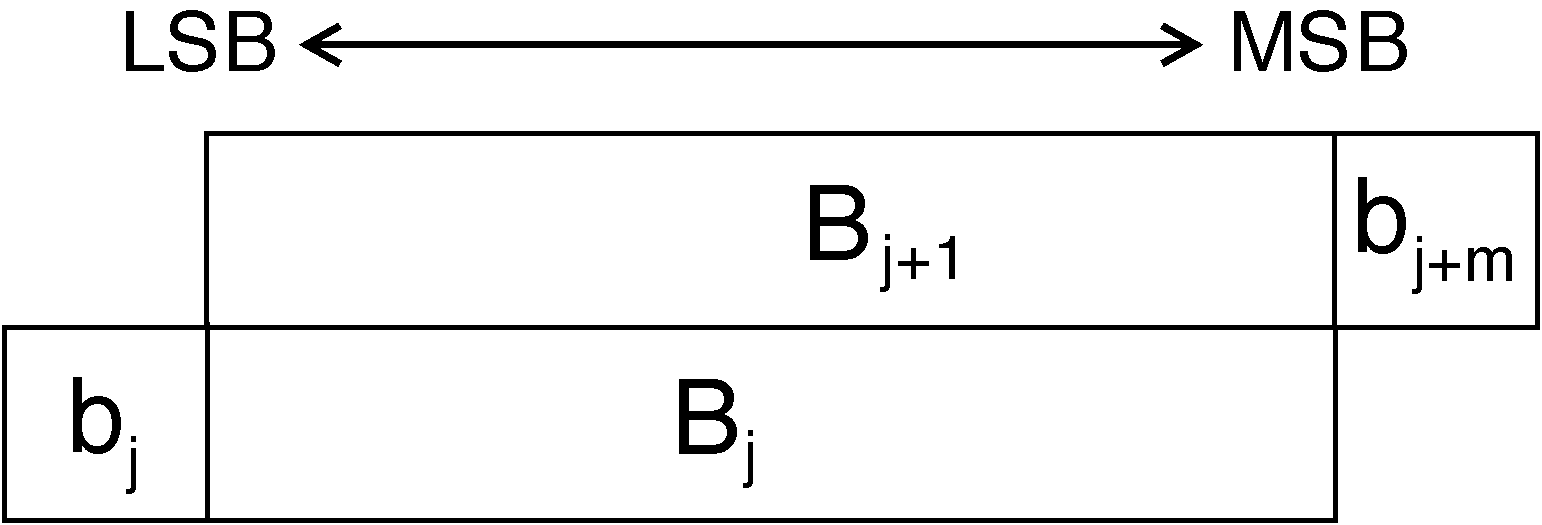
\includegraphics[width=0.3\textwidth]{pattern-matching.pdf}
  \end{center}
  \caption{Pattern Matching bitstrenge. Læg mærke til at LSB og MSB står omvendt af hvordan vi normalt ville læse det, da vi udregner det baglæns.}
  \label{fig:pattern}
\end{figure}

Vi antager at vi kender $B_{j+1}$ Da skal vi starte med at få vores mest signifikante bit $b_{j+m}$ væk, og herefter gange med 2 for at forskyde vores streng med 1. Derefter skal vi blot lægge bit $b_j$ til. Til sidst skal vi køre modulus med $p$. Altså bliver vores formel:

$$
  B_{j} \bmod p
  = \p{2 \p{ B_{j+1} - b_{j+m} 2^{m-1} } + b_j} \bmod p
$$

Således kan vi beregne $B_{n-m}$ i $\O{m}$ tid og herefter alle de resterende $B_j$ frem til $B_0$ i hver $\O{1}$ tid, som giver os en endelig køretid på $\O{n*1 + m} = \O{n}$.



\end{document}
